!TeX root = ../main.tex
% Add the above to each chapter to make compiling the PDF easier in some editors.

\chapter{Previous Literature}\label{chapter:previous literature}

\section{Theoretical Framework}

This chapter discusses the fundamental theories underpinning the study, focusing on portfolio optimization and \ac{GPR}. Understanding these theories is essential for developing the predictive portfolio optimization framework proposed in this research.

\subsection{Portfolio Optimization Theory}

Portfolio optimization is a cornerstone of modern finance, aiming to allocate assets in a way that balances expected returns against risk. The foundational theory in this domain is the \ac{MPT}, introduced by Harry Markowitz in 1952 \cite{markowitz1952portfolio}.

\subsubsection{Modern Portfolio Theory (MPT)}

\ac{MPT} posits that investors can construct an optimal portfolio that offers the maximum expected return for a given level of risk or, equivalently, the minimum risk for a given level of expected return. The key assumptions of MPT are:

\begin{itemize}
    \item Investors are rational and risk-averse, preferring higher returns and lower risk.
    \item Markets are efficient, and all investors have access to the same information.
    \item Asset returns are normally distributed and can be described by their mean (expected return) and variance (risk).
\end{itemize}

\paragraph{Expected Return and Risk}

The expected return of a portfolio, $E[R_p]$, is the weighted sum of the expected returns of the individual assets:

\begin{equation}
    E[R_p] = \sum_{i=1}^{n} w_i E[R_i],
\end{equation}

where $w_i$ is the weight of asset $i$ in the portfolio, $E[R_i]$ is the expected return of asset $i$, and $n$ is the total number of assets.

The portfolio variance, $\sigma_p^2$, representing risk, is given by:

\begin{equation}
    \sigma_p^2 = \sum_{i=1}^{n} \sum_{j=1}^{n} w_i w_j \sigma_{ij},
\end{equation}

where $\sigma_{ij}$ is the covariance between asset $i$ and asset $j$. The standard deviation $\sigma_p$ is the square root of the variance.

\paragraph{Efficient Frontier}

The set of optimal portfolios that offer the highest expected return for a given level of risk forms the \textit{Efficient Frontier}. Portfolios on the efficient frontier are considered optimal, as no other portfolios offer higher returns for the same risk level.

\begin{figure}[h]
    \centering
    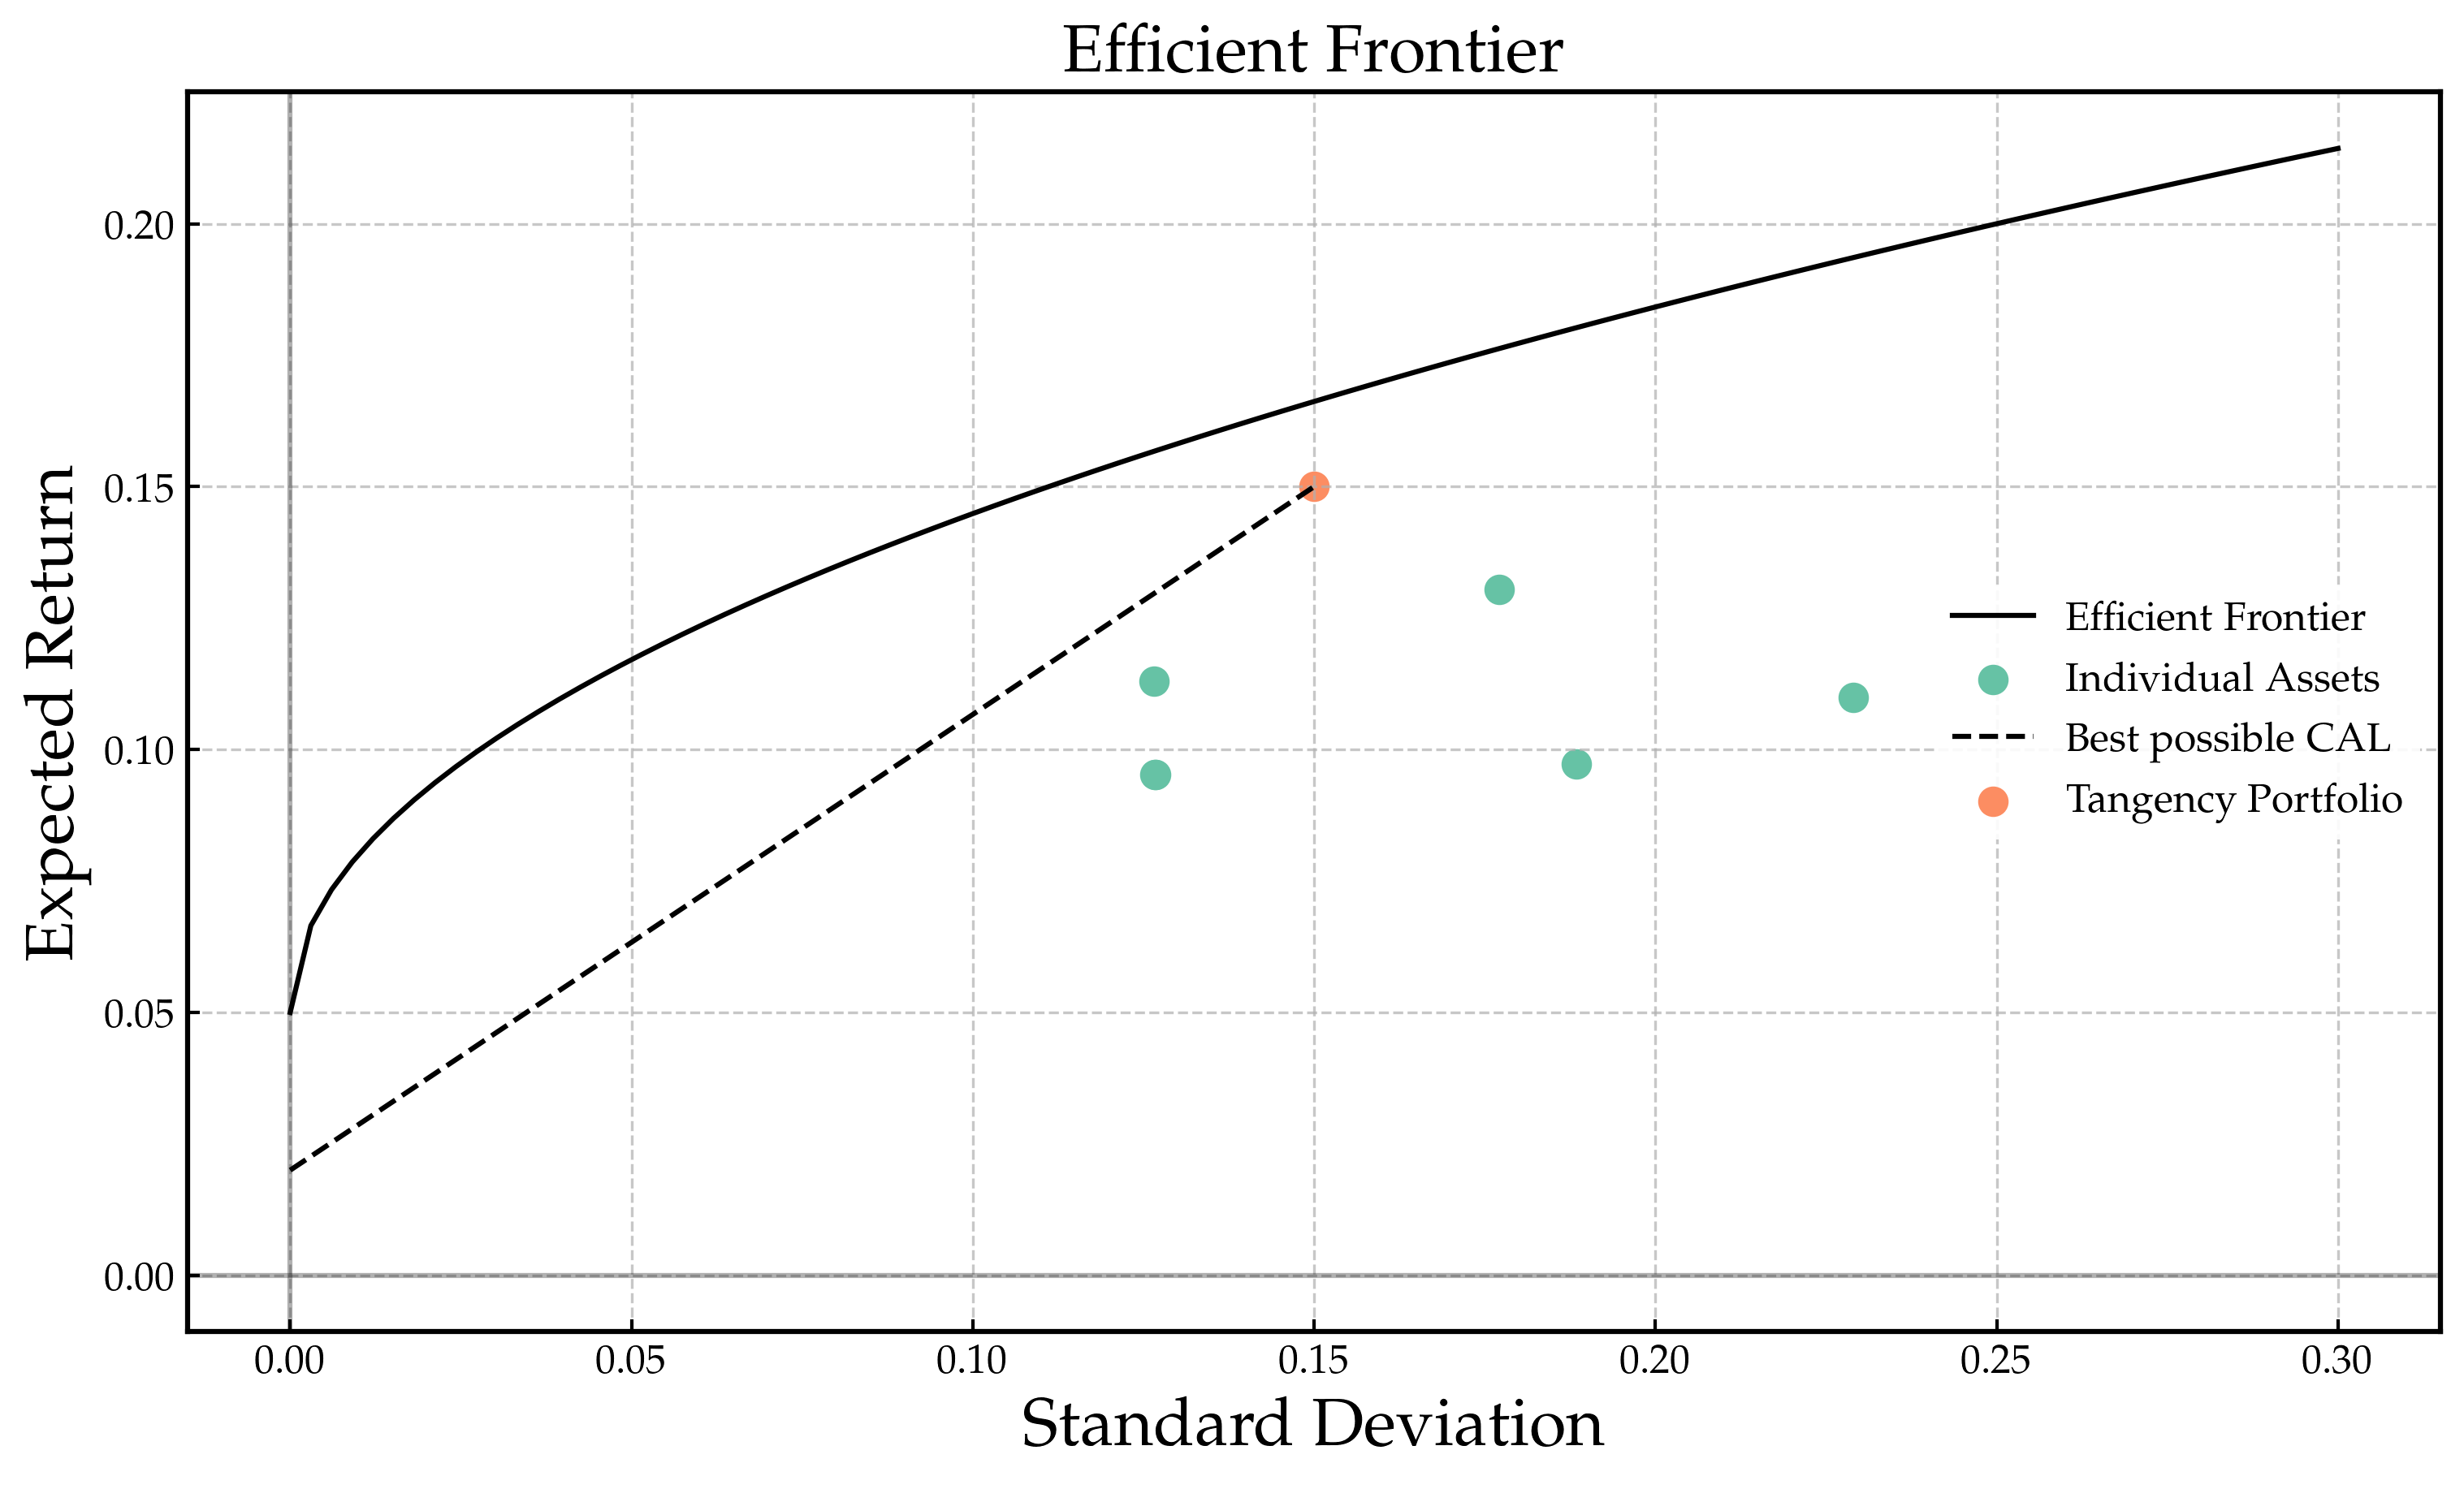
\includegraphics[width=0.6\textwidth]{figures/efficient_frontier.png}
    \caption{Efficient Frontier in Mean-Variance Space}
    \label{fig:efficient_frontier}
\end{figure}

\paragraph{Mean-Variance Optimization}

Mean-variance optimization involves solving for the portfolio weights that minimize the portfolio variance for a given expected return. The optimization problem can be formulated as:

\begin{equation}
\begin{aligned}
    \min_{\mathbf{w}} \quad & \mathbf{w}^T \boldsymbol{\Sigma} \mathbf{w} \\[1ex]
    \text{subject to} \quad & \mathbf{w}^T \mathbf{E} = E_p, \\[1ex]
    & \sum_{i=1}^{n} w_i = 1, \\[1ex]
    & w_i \geq 0, \quad i = 1,\ldots,n,
\end{aligned}
\end{equation}

where:
\begin{itemize}
    \item $\mathbf{w} \in \mathbb{R}^n$ is the vector of asset weights
    \item $\boldsymbol{\Sigma} \in \mathbb{R}^{n \times n}$ is the covariance matrix of asset returns
    \item $\mathbf{E} \in \mathbb{R}^n$ is the vector of expected asset returns
    \item $E_p \in \mathbb{R}$ is the desired expected portfolio return
\end{itemize}
\subsubsection{Risk-Return Trade-off and the Sharpe Ratio}

Investors seek to maximize returns while minimizing risk. The \textit{Sharpe Ratio}, introduced by William F. Sharpe \cite{sharpe1966mutual}, measures the risk-adjusted return of a portfolio:

\begin{equation}
    S = \frac{E[R_p] - R_f}{\sigma_p},
\end{equation}

where $R_f$ is the risk-free rate. A higher Sharpe Ratio indicates a more favorable risk-return trade-off.

\subsubsection{Portfolio Optimization Strategies}

Various strategies exist for portfolio optimization, each with different objectives and constraints:

\begin{itemize}
    \item \textbf{Maximum Return Strategy}: Focuses on maximizing expected returns, often leading to higher risk.
    \item \textbf{Minimum Volatility Strategy}: Aims to minimize risk while achieving a minimum acceptable return.
    \item \textbf{Maximum Sharpe Ratio Strategy}: Seeks the optimal balance between return and risk by maximizing the Sharpe Ratio.
    \item \textbf{Dynamic Strategies}: Adjust portfolio allocations based on changing market conditions and predictive insights.
\end{itemize}

\subsection{Gaussian Process Regression Theory and Applications}

Gaussian Process Regression (GPR) is a non-parametric, Bayesian approach to regression that is particularly powerful for modeling complex, non-linear relationships. GPR provides not only predictions but also uncertainty estimates, which are valuable in risk-sensitive applications like finance.

\subsubsection{Gaussian Processes}

A \textit{Gaussian Process} (GP) is a collection of random variables, any finite number of which have a joint Gaussian distribution \cite{rasmussen2006gaussian}. A GP is fully specified by its mean function $m(\mathbf{x})$ and covariance function $k(\mathbf{x}, \mathbf{x}')$:

\begin{equation}
    f(\mathbf{x}) \sim \mathcal{GP}\left( m(\mathbf{x}), k(\mathbf{x}, \mathbf{x}') \right).
\end{equation}

\paragraph{Mean Function}

The mean function $m(\mathbf{x})$ represents the expected value of the function at point $\mathbf{x}$:

\begin{equation}
    m(\mathbf{x}) = E[f(\mathbf{x})].
\end{equation}

\paragraph{Covariance Function}

The covariance function $k(\mathbf{x}, \mathbf{x}')$ defines the covariance between function values at points $\mathbf{x}$ and $\mathbf{x}'$:

\begin{equation}
    k(\mathbf{x}, \mathbf{x}') = E\left[ (f(\mathbf{x}) - m(\mathbf{x}))(f(\mathbf{x}') - m(\mathbf{x}')) \right].
\end{equation}

Common choices for the covariance function include the squared exponential kernel and the Matérn kernel.

\subsubsection{Gaussian Process Regression for Time-Series Forecasting}

GPR models the underlying function mapping inputs to outputs, capturing uncertainty in predictions. For time-series forecasting:

\begin{itemize}
    \item \textbf{Inputs}: Historical data points, such as lagged returns and time indices.
    \item \textbf{Outputs}: Future values of the time series, such as asset returns.
\end{itemize}

Given training data $\{ (\mathbf{x}_i, y_i) \}_{i=1}^N$, where $\mathbf{x}_i$ are inputs and $y_i$ are observations, the goal is to predict the output $f_*$ at a new input $\mathbf{x}_*$.

\paragraph{Predictive Distribution}

The predictive distribution of $f_*$ given the training data is Gaussian:

\begin{equation}
    p(f_* | \mathbf{x}_*, \mathbf{X}, \mathbf{y}) = \mathcal{N}\left( f_* | \mu_*, \sigma_*^2 \right),
\end{equation}

where

\begin{equation}
    \mu_* = k_*^\top (\mathbf{K} + \sigma_n^2 \mathbf{I})^{-1} \mathbf{y}, \\
    \sigma_*^2 = k(\mathbf{x}_*, \mathbf{x}_*) - k_*^\top (\mathbf{K} + \sigma_n^2 \mathbf{I})^{-1} k_*.
\end{equation}
Here, $k_* = [k(\mathbf{x}_*, \mathbf{x}_1), \dots, k(\mathbf{x}_*, \mathbf{x}_N)]^\top$, $\mathbf{K}$ is the covariance matrix with entries $K_{ij} = k(\mathbf{x}_i, \mathbf{x}_j)$, and $\sigma_n^2$ is the noise variance.

\subsubsection{Covariance Functions (Kernels)}

The choice of kernel function $k(\mathbf{x}, \mathbf{x}')$ is critical in GPR as it encodes assumptions about the function being learned.


\begin{itemize}
    \item \textit{Squared Exponential Kernel}:

    \begin{equation}
        k_{\text{SE}}(\mathbf{x}, \mathbf{x}') = \sigma_f^2 \exp\left( -\frac{1}{2\ell^2} ||\mathbf{x} - \mathbf{x}'||^2 \right),
    \end{equation}

    where $\sigma_f^2$ is the signal variance and $\ell$ is the length-scale parameter.

    \item \textit{Matérn Kernel}:

    \begin{equation}
        k_{\text{Matérn}}(\mathbf{x}, \mathbf{x}') = \sigma_f^2 \frac{2^{1-\nu}}{\Gamma(\nu)} \left( \frac{\sqrt{2\nu}||\mathbf{x} - \mathbf{x}'||}{\ell} \right)^\nu K_\nu\left( \frac{\sqrt{2\nu}||\mathbf{x} - \mathbf{x}'||}{\ell} \right),
    \end{equation}

    where $\nu$ controls the smoothness, $\Gamma$ is the gamma function, and $K_\nu$ is the modified Bessel function.

\end{itemize}

\subsubsection{Gaussian Process Regression for Time-Series Forecasting}

In GPR, given training data $\{ (\mathbf{x}_i, y_i) \}_{i=1}^n$, the goal is to predict the output $y_*$ for a new input $\mathbf{x}_*$. The predictive distribution is Gaussian with mean and variance:

\begin{equation}
    E[y_*] = \mathbf{k}_*^T (\mathbf{K} + \sigma_n^2 \mathbf{I})^{-1} \mathbf{y},
\end{equation}

\begin{equation}
    \text{Var}[y_*] = k_{**} - \mathbf{k}_*^T (\mathbf{K} + \sigma_n^2 \mathbf{I})^{-1} \mathbf{k}_*,
\end{equation}

where:

\begin{itemize}
    \item $\mathbf{K}$ is the $n \times n$ covariance matrix evaluated at the training inputs.
    \item $\mathbf{k}_*$ is the covariance vector between the test point and the training inputs.
    \item $k_{**}$ is the covariance between the test point and itself.
    \item $\sigma_n^2$ is the variance of the observation noise.
    \item $\mathbf{y}$ is the vector of training targets.
\end{itemize}

\paragraph{Advantages of GPR in Financial Modeling}

GPR offers several benefits for financial time-series forecasting:

\begin{itemize}
    \item \textit{Non-parametric Flexibility}: Does not assume a specific functional form, allowing for modeling of complex, non-linear relationships.
    \item \textit{Uncertainty Quantification}: Provides probabilistic predictions with associated confidence intervals, which are crucial for risk management.
    \item \textit{Bayesian Framework}: Naturally incorporates prior knowledge and updates beliefs with new data.
\end{itemize}

\subsubsection{Challenges in Applying GPR to Finance}

Despite its advantages, GPR faces challenges in financial applications:

\begin{itemize}
    \item \textit{Computational Complexity}: Involves inverting an $n \times n$ matrix, which can be computationally intensive for large datasets.
    \item \textit{Non-Stationarity}: Financial time-series often exhibit non-stationary behavior, violating assumptions of stationarity in standard GPR.
    \item \textit{Noise Characteristics}: Financial data can be noisy and volatile, affecting model performance.
    \item \textit{Hyperparameter Tuning}: Selection of kernel functions and hyperparameters significantly impacts model performance and requires careful tuning.
\end{itemize}


\subsection{Integrating Portfolio Optimization and GPR}

Combining portfolio optimization with GPR-based forecasting aims to leverage accurate predictions of asset returns and associated uncertainties to make informed allocation decisions. The integration involves:

\begin{itemize}
    \item Using GPR to predict expected returns and volatilities for assets.
    \item Incorporating these predictions into the optimization models to determine optimal portfolio weights.
    \item Adjusting for uncertainties by considering the confidence intervals provided by GPR in the optimization process.
\end{itemize}

\paragraph{Dynamic Portfolio Optimization}

Dynamic optimization involves updating the portfolio allocation as new information becomes available. By retraining the GPR models with new data and adjusting the portfolio accordingly, the strategy adapts to changing market conditions, potentially enhancing performance.

\subsection{Conclusion}

The theoretical foundation provided by portfolio optimization theory and Gaussian Process Regression is critical for developing the predictive portfolio optimization framework. Understanding the principles, advantages, and limitations of these theories allows for effective integration and application in financial modeling and asset allocation.


\section{Risk measures and portfolio optimization}

\section{Machine Learning in Financial Markets}

\subsection{Overview of Machine Learning Applications in Finance}

The financial markets generate vast amounts of data daily, encompassing stock prices, trading volumes, economic indicators, and news articles. Machine learning algorithms are uniquely positioned to process and analyze this data, uncovering patterns and insights that traditional statistical methods may overlook. Key applications of machine learning in finance include:

\subsubsection{Time-Series Forecasting}

Predicting future asset prices and market trends is a fundamental objective in finance. Machine learning models, such as neural networks, support vector machines, and ensemble methods, are employed to forecast time-series data by capturing non-linear relationships and complex temporal dependencies \cite{sezer2020financial}.

\subsubsection{Algorithmic Trading}

Machine learning algorithms facilitate the development of automated trading systems that execute trades based on predefined strategies and real-time data analysis. Techniques like reinforcement learning enable the optimization of trading strategies through continuous learning from market interactions \cite{nevmyvaka2006reinforcement}.

\subsubsection{Risk Management}

Accurate risk assessment is crucial for financial institutions. Machine learning models help in predicting credit risk, market risk, and operational risk by analyzing historical data and identifying factors that contribute to potential losses \cite{lessmann2015benchmarking}.

\subsubsection{Portfolio Optimization}

Machine learning enhances portfolio optimization by providing more accurate estimates of expected returns and covariances between assets. Advanced models can adapt to changing market conditions and incorporate a broader set of predictive features \cite{heaton2017deep}.

\subsubsection{Fraud Detection and Anomaly Detection}

Detecting fraudulent activities and anomalies is vital for maintaining the integrity of financial systems. Machine learning algorithms, particularly unsupervised learning techniques, are used to identify unusual patterns in transaction data that may indicate fraud \cite{phua2010comprehensive}.

\subsubsection{Sentiment Analysis and Natural Language Processing}

Analyzing news articles, social media, and financial reports using natural language processing (NLP) helps investors gauge market sentiment and its potential impact on asset prices \cite{hagenau2013automated}.


\subsection{Conclusion}

Machine learning plays a pivotal role in modern financial analysis, offering sophisticated tools for modeling and decision-making. Gaussian Process Regression, with its probabilistic nature and flexibility, is particularly well-suited for financial applications that require modeling uncertainty and non-linear relationships. Understanding the theoretical foundations and practical considerations of GPR is essential for its effective integration into financial modeling and portfolio optimization.


\section{Dynamic Portfolio Management}

Dynamic portfolio management involves continuously adjusting asset allocations in response to changing market conditions, forecasts, and investment objectives. Unlike static strategies, dynamic approaches aim to optimize the portfolio over time by incorporating new information and adapting to market dynamics. This section reviews dynamic optimization strategies, discusses the impact of transaction costs on portfolio rebalancing, and examines existing approaches to strategy switching.

\subsection{Review of Dynamic Optimization Strategies}

Dynamic optimization strategies are designed to adapt portfolio allocations over time, taking into account the stochastic nature of asset returns and changing investment opportunities. Key concepts and methods in dynamic portfolio optimization include:

\subsubsection{Dynamic Programming}

Dynamic programming is a mathematical optimization approach that solves complex problems by breaking them down into simpler subproblems. In the context of portfolio optimization, dynamic programming can be used to determine the optimal investment policy over multiple periods \cite{bellman1957dynamic}.

\paragraph{Bellman's Principle of Optimality}

Bellman's principle states that an optimal policy has the property that, whatever the initial state and initial decision are, the remaining decisions must constitute an optimal policy with regard to the state resulting from the first decision. This principle underpins dynamic programming methods in portfolio optimization.

\subsubsection{Stochastic Control Theory}

Stochastic control theory deals with decision-making in systems that evolve over time under uncertainty. In portfolio optimization, stochastic control models can determine optimal asset allocations by considering the stochastic processes governing asset returns and investor wealth \cite{merton1969lifetime}.

\paragraph{Merton's Portfolio Problem}

Robert C. Merton extended the continuous-time portfolio optimization framework by incorporating stochastic control techniques. Merton's model determines the optimal consumption and portfolio allocation strategies for an investor with a finite or infinite investment horizon, maximizing expected utility \cite{merton1971optimum}.

\subsubsection{Reinforcement Learning}

Reinforcement learning (RL) is a machine learning paradigm where agents learn optimal policies through interactions with the environment by maximizing cumulative rewards. In finance, RL can be applied to portfolio management by treating asset allocation as a sequential decision-making problem \cite{moody1998performance}.

\paragraph{Applications in Portfolio Management}

RL algorithms, such as Q-learning and policy gradients, have been used to develop adaptive trading strategies that learn from market data and adjust allocations dynamically \cite{almahdi2019adaptive}.

\subsubsection{Scenario Analysis and Model Predictive Control}

Scenario analysis involves evaluating portfolio performance under different hypothetical future states of the world. Model Predictive Control (MPC) uses forecasts to optimize current decisions while considering future trajectories, adjusting strategies as new information becomes available \cite{primbs2009dynamic}.

\paragraph{Advantages of MPC}

MPC allows for the incorporation of predictive models (e.g., GPR forecasts) into the optimization process, enabling the portfolio to adapt dynamically to anticipated market changes.

\subsection{Transaction Costs and Portfolio Rebalancing}

Transaction costs play a significant role in dynamic portfolio management, as frequent rebalancing can erode returns. Understanding and modeling transaction costs are essential for effective portfolio optimization.

\subsubsection{Types of Transaction Costs}

Transaction costs can be broadly categorized into:

\begin{itemize}
    \item \textit{Fixed Costs}: Costs that are constant per transaction, such as brokerage fees.
    \item \textit{Variable Costs}: Costs that depend on the transaction size, including bid-ask spreads and market impact.
    \item \textit{Slippage}: The difference between the expected transaction price and the actual execution price.
\end{itemize}

\subsubsection{Impact on Portfolio Performance}

High transaction costs can negate the benefits of frequent rebalancing. Incorporating transaction costs into the optimization model encourages more conservative adjustments, potentially leading to better net performance \cite{garleanu2009dynamic}.

\subsubsection{Optimal Rebalancing Frequency}

Determining the optimal frequency of portfolio rebalancing involves a trade-off between maintaining the desired asset allocation and minimizing transaction costs. Strategies to address this include:

\begin{itemize}
    \item \textit{Threshold-Based Rebalancing}: Rebalancing only when asset weights deviate beyond predefined thresholds.
    \item \textit{Periodic Rebalancing}: Adjusting the portfolio at regular intervals (e.g., monthly, quarterly).
    \item \textit{Cost-Aware Optimization}: Incorporating transaction costs directly into the optimization problem to balance expected returns against costs.
\end{itemize}

\subsection{Existing Approaches to Strategy Switching}

Strategy switching involves changing between different portfolio optimization strategies based on market conditions, forecasts, or performance metrics. This adaptive approach seeks to capitalize on the strengths of various strategies under different scenarios.

\subsubsection{Regime-Switching Models}

Regime-switching models assume that financial markets alternate between different states or regimes (e.g., bull and bear markets). By identifying the current regime, investors can switch to strategies that are better suited to prevailing conditions \cite{ang2002regime}.

\paragraph{Markov Switching Models}

These models use Markov processes to model transitions between regimes, allowing for probabilistic predictions of future states and informing strategy selection \cite{hamilton1989new}.

\subsubsection{Meta-Learning and Ensemble Methods}

Meta-learning approaches involve training a higher-level model to select the best-performing strategy from a set of candidates. Ensemble methods combine multiple strategies to create a more robust overall strategy \cite{huang2019building}.

\paragraph{Performance-Based Selection}

Strategies can be evaluated based on historical or real-time performance metrics, such as Sharpe ratios or drawdowns, with the best-performing strategy selected for implementation \cite{poterba2000portfolio}.

\subsubsection{Rule-Based Switching}

Rule-based systems use predefined criteria or indicators to trigger strategy changes. Examples include:

\begin{itemize}
    \item \textit{Technical Indicators}: Switching strategies based on signals from moving averages, momentum indicators, or relative strength indexes.
    \item \textit{Economic Indicators}: Adjusting strategies in response to macroeconomic data releases or changes in interest rates.
    \item \textit{Forecast Confidence}: Modifying the strategy based on the confidence level of predictive models, such as forecast variances from GPR.
\end{itemize}

\subsubsection{Machine Learning-Based Switching}

Machine learning models can be trained to predict the optimal strategy based on market data and indicators. Classification algorithms, such as support vector machines or neural networks, can identify patterns associated with the outperformance of specific strategies \cite{fernandez2018machine}.

\subsection{Conclusion}

Dynamic portfolio management seeks to enhance investment performance by adapting to market conditions and new information. Incorporating transaction costs into the optimization process is crucial for realistic strategy implementation. Existing approaches to strategy switching provide valuable frameworks for developing adaptive strategies, leveraging techniques such as regime-switching models, meta-learning, rule-based systems, and machine learning. This study builds upon these concepts by introducing a probabilistic, threshold-based strategy switching mechanism informed by Gaussian Process Regression forecasts.




